\documentclass[12pt]{article}
\usepackage{graphicx,import}
\usepackage{float}
\usepackage[svgnames]{xcolor} 
\usepackage{makecell}
\usepackage{fancyhdr}
\usepackage{subcaption}
\usepackage{hyperref}
\usepackage{enumitem}
\usepackage[many]{tcolorbox}
\usepackage{listings }
\usepackage[a4paper, total={6in, 8in} , bottom = 25mm , top = 25mm, headheight = 1.25cm , includehead,includefoot,heightrounded ]{geometry}
\usepackage{afterpage}
\usepackage{amssymb}
\usepackage{pdflscape}
\usepackage{gensymb}
\usepackage{textcomp}
\usepackage{tikz,pgfplots}
\usepackage{xecolor}
\usepackage{rotating}
\usepackage{pdfpages}
\usepackage[Kashida]{xepersian}
\usepackage[T1]{fontenc}
\usepackage{tikz}
\usepackage[utf8]{inputenc}
\usepackage{PTSerif} 
\usepackage{seqsplit}
\usepackage{hhline}
\usepackage{pgfgantt}
\usepackage{graphicx}
\usepackage{filecontents}
\usepackage{url} % for "\url" macro
\usepackage{babel}
\usepackage[backend=bibtex, style=numeric]{biblatex}

\addbibresource{refs.bib}

\graphicspath{ {./images/} }

\renewcommand\theadalign{bc}
\renewcommand\theadfont{\bfseries}
\renewcommand\theadgape{\Gape[4pt]}
\renewcommand\cellgape{\Gape[4pt]}

\usepackage[edges]{forest}

\usepackage{listings}
\usepackage{xcolor}

\hypersetup{
	colorlinks   = true, %Colours links instead of ugly boxes
	urlcolor     = blue, %Colour for external hyperlinks
	linkcolor    = blue, %Colour of internal links
	citecolor   = red %Colour of citations
}
 
\definecolor{codegreen}{rgb}{0,0.6,0}
\definecolor{codegray}{rgb}{0.5,0.5,0.5}
\definecolor{codepurple}{rgb}{0.58,0,0.82}
\definecolor{backcolour}{rgb}{0.95,0.95,0.92}
 
\NewDocumentCommand{\codeword}{v}{
\texttt{\textcolor{blue}{#1}}
}
\lstset{language=java,keywordstyle={\bfseries \color{blue}}}


\lstdefinestyle{mystyle}{
    backgroundcolor=\color{backcolour},   
    commentstyle=\color{codegreen},
    keywordstyle=\color{magenta},
    numberstyle=\tiny\color{codegray},
    stringstyle=\color{codepurple},
    basicstyle=\ttfamily\normalsize,
    breakatwhitespace=false,         
    breaklines=true,                 
    captionpos=b,                    
    keepspaces=true,                 
    numbers=left,                    
    numbersep=5pt,                  
    showspaces=false,                
    showstringspaces=false,
    showtabs=false,                  
    tabsize=2
}

\lstset{style=mystyle}

\settextfont[Scale=1.2, Path = fonts/ ,BoldFont={Bahij Nazanin-Bold} , ItalicFont = {IRNazaninIranic}]{Bahij Nazanin-Regular}
% \setlatintextfont[Scale = 1.0, Path = fonts/]{Garamond}
% \DefaultMathsDigits 
\DeclareMathSizes{11}{19}{13}{9} 
%\DeclareMathSizes{12}{14.4}{8}{9}





\newenvironment{changemargin}[2]{%
\begin{list}{}{%
\setlength{\topsep}{0pt}%
\setlength{\leftmargin}{#1}%
\setlength{\rightmargin}{#2}%
\setlength{\listparindent}{\parindent}%
\setlength{\itemindent}{\parindent}%
\setlength{\parsep}{\parskip}%
}%
\item[]}{\end{list}}


\definecolor{foldercolor}{RGB}{124,166,198}

\tikzset{pics/folder/.style={code={%
    \node[inner sep=0pt, minimum size=#1](-foldericon){};
    \node[folder style, inner sep=0pt, minimum width=0.3*#1, minimum height=0.6*#1, above right, xshift=0.05*#1] at (-foldericon.west){};
    \node[folder style, inner sep=0pt, minimum size=#1] at (-foldericon.center){};}
    },
    pics/folder/.default={20pt},
    folder style/.style={draw=foldercolor!80!black,top color=foldercolor!40,bottom color=foldercolor}
}

\forestset{is file/.style={edge path'/.expanded={%
        ([xshift=\forestregister{folder indent}]!u.parent anchor) |- (.child anchor)},
        inner sep=1pt},
    this folder size/.style={edge path'/.expanded={%
        ([xshift=\forestregister{folder indent}]!u.parent anchor) |- (.child anchor) pic[solid]{folder=#1}}, inner xsep=0.6*#1},
    folder tree indent/.style={before computing xy={l=#1}},
    folder icons/.style={folder, this folder size=#1, folder tree indent=3*#1},
    folder icons/.default={12pt},
}

\begin{document}


%%% title pages
\begin{titlepage}
\begin{center}
        
\vspace*{0.7cm}


\includegraphics[width=0.4\textwidth]{sharif1.png}\\
\vspace{0.5cm}
\textbf{ \Huge{\emph ‌آزمایشگاه سخت‌افزار} }\\
\vspace{0.5cm}
\textbf{ \Large{گزارش فاز اول} }
\vspace{0.2cm}
       
 
      \large \textbf{دانشکده مهندسی کامپیوتر}\\\vspace{0.2cm}
    \large   دانشگاه صنعتی شریف\\\vspace{0.2cm}
       \large   ﻧﯿﻢ سال اول 02-01 \\\vspace{0.2cm}
      \noindent\rule[1ex]{\linewidth}{1pt}
استاد:\\
    \textbf{{جناب آقای دکتر اجلالی}}


دستیار آموزشی:\\
\textbf{{جناب آقای دکتر فصحتی}}

    \vspace{0.25cm}
    
    موضوع پروژه:\\
    
    \textbf{دید در شب اتومبیل}
    
    \vspace{0.35cm}
    
    
        شماره گروه:
    \textbf{{۶}}\\
    
اعضای گروه:\\

    \textbf{{علیرضا شاطری}}
    \\
   
     \textbf{{رضا امینی}}   
\end{center}
\end{titlepage}
%%% title pages


%%% header of pages
\newpage
\pagestyle{fancy}
\fancyhf{}
\fancyfoot{}
\cfoot{\thepage}
\chead{}
\rhead{
\includegraphics[width=0.1\textwidth]{sharif.png}}
\lhead{گزارش فاز اول}
%%% header of pages

\newfontfamily\terminal{Courier New Bold}

\KashidaOff
 \newcommand{\inlineLatin}[1]{
	\small{\lr{{\terminal #1}}}
}


\tableofcontents
\listoffigures
\listoftables

\newpage
\section{مقدمه}

محصول نهایی این پروژه، یک سیستم دید در شب است که درون اتومبیل قرار می‌گیرد و به راننده در هنگام رانندگی در تاریکی، کمک به سزایی می‌کند. در این سیستم اطلاعات از طریق یک دوربین حرارتی به ماژول رزپری منتقل می‌شود و کدهایی که در رزپری قرار داده شده است با انجا پردازش تصویری ساده، تشخیص خواهد داد که آیا موجود زنده‌ای در میدان دید راننده حضور دارد یا خیر. همچنین از طریق چراغ و صدا نتیجه را به راننده اطلاع می‌دهد.
\\

در این فاز ما قطعات را تهیه کردیم، آشنایی اولیه‌ای با رزپری به دست آوردیم، مقایسه‌ای مختصر از دو ماژول دوربین حرارتی و دوربین دید در شب داشتیم و روش‌های تست محصول را نیز طراحی نمودیم. در این مستند به ارائه گزارش هر یک از اقدامات اشاره شده می‌پردازیم.

\section{گزارش انجام پروژه}
\subsection{تهیه قطعات}

لیست قطعات تهیه شده به همراه قیمت تخمینی و قیمت تهیه‌شده در جدول زیر قابل مشاهده است:

\begin{table}[h]
	\begin{tabular}{|c|c|c|c|}
		\hline
		\textbf{ردیف} &
		\textbf{قطعه} &
		\textbf{\begin{tabular}[c]{@{}c@{}}قیمت کل\\  تخمین‌زده شده\\ (هزار تومان)\end{tabular}} &
		\textbf{\begin{tabular}[c]{@{}c@{}}قیمت کل نهایی\\ (هزار تومان)\end{tabular}} \\ \hline
		۱  & رزپری پای & \lr{3100}   & \lr{0*}  \\ \hline
		۲ &
		\begin{tabular}[c]{@{}c@{}}دوربین حرارتی\end{tabular} &
		\lr{1100} &
		\lr{1100} \\ \hline
		۳  & USB Flash   & \lr{100}     & \lr{0*}    \\ \hline
		۴ & LED and Board                               & \lr{50}     & \lr{0*}     \\ \hline
		& \textbf{مجموع}                       & \lr{4350} & \lr{1100} \\ \hline
	\end{tabular}
	\caption{هزینه‌ها}
\end{table}

قطعاتی که کنار قیمت نهایی آن‌ها علامت * وجود دارد، به علت موجود بودن خریداری نشده‌اند و قیمت نهایی آن‌ها صفر در نظر گرفته شده است.


هزینه تخمین‌زده شده‌ی اولیه‌ی ما ۴۳۵۰ هزارتومان بود اما با توجه به موجود بودن قطعات، تنها قطعه‌ی دوربین حرارتی نیاز به خرید داشته و جداگانه تهیه شده است.


\subsection{آشنایی با رزبری‌پای}

\subsubsection{معرفی رزبری‌پای }

رزپری‌پای در واقع یک کامپیوتر کامل است که در ابعاد کوچکتر و با منابع محدودتری ساخته شده است. اما با وجود این محدودیت‌ها همچنان مانند یک کامپیوتر واقعی امکان اتصال به مانیتور، ماوس، کیبرد، اسپیکر و خیلی از دیوایس‌های دیگر را دارد.

\begin{figure}[h]
	\begin{center}
		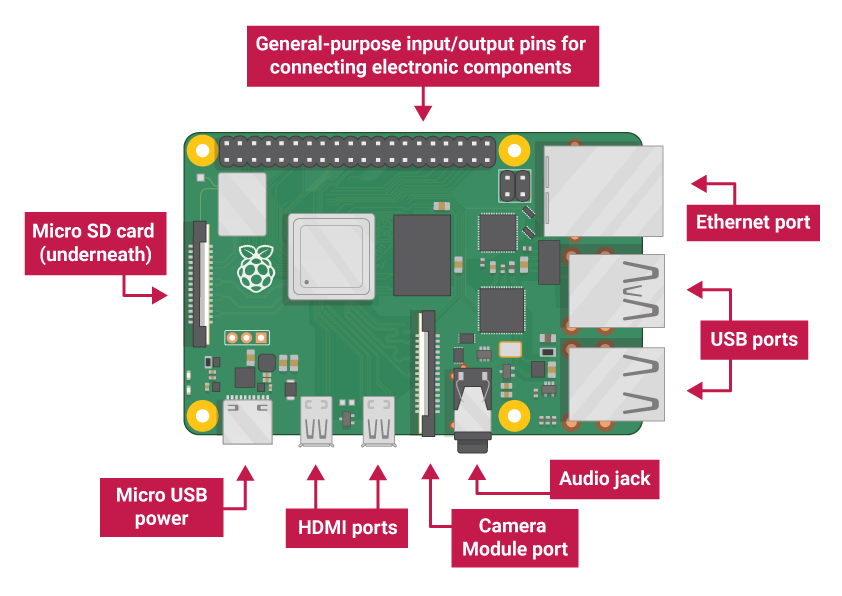
\includegraphics[width=.50\textwidth]{pi-labelled-names}
	\end{center}
	\caption{قسمت‌های مختلف رزبری}
\end{figure}


 رزپری از قسمت‌های مختلفی تشکیل شده است که موارد زیر را شامل می‌شود:
 \\
 
\begin{itemize}
	\item 
	پورت‌های \lr{USB}:  جهت اتصال ماوس، کیبورد، درایو USB و ...
	\item 
	
	جایگاه \lr{SD card}: محل قرارگیری کارت SD که شامل سیستم‌عامل و سایر فایل‌ها می‌شود.
	\item 
	
	پورت اترنت: جهت اتصال رزبری به شبکه
	
	\item 
	جک صدا: جهت اتصال هندزفری و ...
	\item 
	
	پورت\lr{HDMI}:  جهت اتصال به مانیتور
	\item 
رابط منبع تغذیه: جهت اتصال رزبری به منبع تغذیه
	
	\item
	پین‌های\lr{GPIO}: 
	 ۴۰ پین ورودی/خروجی همه منظوره که با استفاده از این پین‌ها می‌توان قطعات مختلف الکترونیکی مانند سنسورها و موتورها را به رزبری متصل کرد.
\end{itemize}




\begin{figure}[h]
	\begin{center}
		\includegraphics[width=.50\textwidth]{pi3_5F00_gpio}
	\end{center}
	\caption{پین‌های GPIO رزبری‌پای ۳}
\end{figure}



\subsubsection{‌راه‌اندازی رزبری‌پای}

کار کردن با رزپری‌پای نیاز به سیستم عامل اختصاصی خودش را دارد. این سیستم عامل که 
\lr{Raspberry Pi OS} نام دارد بر پایه‌ی کرنل لینوکس توسعه داده شده و بهینه سازی شده برای محیط‌هایی با منابع محاسباتی محدود است.
 پس در قدم اول باید این سیستم عامل را روی رزپرری‌پای نصب کنیم. برای این کار کافی‌ست \lr{MicroSD} را داخل لپتاپ خود قرار دهیم و با کمک برنامه‌ی \lr{Raspberry Pi Imager} سیستم را روی آن رایت کنیم.
 \\
 
 در مرحله‌ی بعد کافی‌ست این \lr{MicroSD} را به رزپری متصل کرده و رزپری را روشن کنیم. اگر چراغ سبز رزپری چشمک بزند یعنی سیستم با موفقت بوت شده و قابل استفاده است. حال می‌توان آن را به مانیتور وصل کرده و به کمک کیبرد و موس با آن کار کنیم.

\newpage
\subsection{انتخاب بین دو طراحی}
همانطور که در پروپوزال پروژه اشاره کرده بودیم، دو راه برای طراحی محصول نهایی در جلوی راهمان قرار داشت. یکی استفاده از دوربین حرارتی و دیگری استفاده از دوربین دید در شب. هر کدام از این دوربین‌ها مزایا و معایب خاص خودشان را دارند که در اینجا به آن‌ها بررسی می‌کنیم:

\subsubsection{دوربین حرارتی}

مزایا:

\begin{itemize}
    \item ارزان
    \item وجود کد‌هایی که از قبل روی آن زده شده
    \item پین‌های کمتر در نتیجه کاربرد ساده‌تر
\end{itemize}
\\
معایب:

\begin{itemize}
    \item دقت پایین
    \item تک کاربرده
\end{itemize}

\subsubsection{دوربین دید در شب}

مزایا:

\begin{itemize}
    \item کاربرد‌های زیاد (یعنی می‌توان بر بستر آن فیچرهای دیگری نیز ارائه داد)
    \item دقت و کیفیت بسیار بالا
    \item مدرن‌تر و پیشرفته‌تر
    \item امکان اندازه گیری فاصله تا موجود زنده
\end{itemize}
\\
معایب:

\begin{itemize}
    \item گران
    \item مستندات اندک (تقریبا هیچ کد توسعه داده شده‌ای هم یافت نشد)
    \item پین‌ها و امکانات زیاد در نتیجه کاربرد دشوارتر
\end{itemize}

در نهایت با کنار هم قرار دادن تمام مزایا و معایب و با توجه به این که هدف این پروژه بیشتر آموزشی‌ست و باید زمان و هزینه را به خوبی مدیریت کرد، تصمیم گرفتیم تا از ماژول دوربین حرارتی با وجود کاستی‌هایی، استفاده کنیم. این ماژول نیاز ما را در محیطی آزمایشگاهی برطرف کرده و برای طراحی یک مدل MVP از محصول نهایی بسیار مفید است. 
در نتیجه ما دوربین حرارتی را تهیه نموده و در حال تست و اجرای کد روی آن هستیم تا به نتیجه دلخواه برسیم.

\subsection{سناریو تست محصول}
برای تست این محصول، تنها مرحله‌ای که می‌توان سناریو‌های مختلف را روی آن پیاده کرد، بعد از اتمام پیاده‌سازی اولیه است. در برنامه‌ای که در حال حاضر در نظر گرفته‌ایم تا ۲ آذر این پیاده‌سازی را به طور کامل تمام کنیم. سپس سناریو‌های زیر را روی محصول اجرا می‌کنیم:

\begin{itemize}
    \item تست ماژول دوربین حرارتی: در این تست سیستم را در محیطی تاریک قرار می‌دهیم سپس از طریق قطعه کدی که روی رزپری اجرا شده است، هرگاه جسمی با حرارت بالاتر از حد معین در میدان دید دوربین ظاهر شد، لاگ می‌اندازیم تا متوجه درستی کارکرد دوربین بشویم.
    
    \item تست چراغ‌های LED: حال همان تست قبلی را این بار با روشن کردن چراغ‌های قرمز انجام می‌دهیم. هرگاه موجود زنده‌ای شناسایی شد چرا‌غ‌های قرمز خطر روشن شود.
    
    \item روشن شدن چراغ‌های LED که در راستای موجود زنده قرار دارند: در این تست علاوه بر تست‌های قبلی عملکرد چراغ‌های راهنما هم تست می‌شود. یعنی چراغ‌هایی که باید در چهت حضور موجود زنده روشن شوند و چراغ‌هایی که در جهت آن نیستند باید خاموش باقی بمانند.
    
    \item تست تاریخچه‌ی شناسایی‌های قبلی: در این تست نیز باید ابتدا تست سوم چندین بار تکرار شود و در نهایت لاگ‌ها ثبت شده در حافظه را بررسی کرد و درستی آن‌ها را تایید نمود.
\end{itemize}

نکته‌ای که باید در همه تست‌های بالا رعایت شود کم نور بودن محیط است. همچنین تست‌ها را به صورت incremental در نظر گرفته‌ایم. یعنی آن‌ها را باید به ترتیب انجام دهیم و هرگاه به تست آخر رسیدیم و نتیجه درستی از آن گرفتیم، می‌توانیم بگوییم که محصول دارد به درستی کامل کار می‌کند.


\end{document}

